In this section we briefly summarise the results of the ML analysis performed
on the data.
We will explore several diverse algorithms including regularised versions of
the linear regression (LR, from now on), support vector machines (SVM),
decision trees (random forests, RF, and gradient boosted decision trees, GBDT),
and artificial neural networks (ANN).
For each algorithm we fit the data on training set and evaluate it on the
validation set to perform the optimisation of the \textit{hyperparameters}
using Bayes
statistics~(see
\cite{Pedregosa:2011:ScikitLearn,Head:2018:ScikitOptimize,Ke:2017:LightGBM,Abadi:2015:TensorFlow}
for the modules used in the analysis: \texttt{scikit-learn} for linear models
and SVM, \texttt{lightgbm} for trees and \texttt{tensorflow} for the ANN).
The goal is to minimise the objective function, that is the validation MSE,
without knowing its analytic form, by only inferring the probability of
obtaining a better result with a different choice of hyperparameters.

\subsection{Regression Analysis}\label{sec:ml:regr}

In \Cref{tab:ml:test} we summarise the results obtained from prediction on the
test set for the algorithms used: in particular the first four lines refer to
linear models (LR is the plain regression, EN implements both $\ell_1$ and
$\ell_2$ linear regularisation (i.e.\ it introduces in the linear least square
minimisation terms proportional to the norm and the squared norm of the
parameters of the fit, weighted by two separate terms), Lasso and Ridge
separately implement $\ell_1$ and $\ell_2$ regularisation, respectively); l-SVR
is the linear implementation of the SVM models, while r-SVR uses a Gaussian
\textit{kernel trick}; RF and GBDT are different ensemble algorithms based on
decision trees (namely random forests and gradient boosted trees); ANN
represents the neural network architecture (no hidden layers, only one input
layer with 30 units, batch normalisation layer and a dropout layer with 0.1
drop rate leading to a network of 691 trainable parameters and 60 fixed
parameters).

\begin{table}[htbp]
\centering
\resizebox{0.475\textwidth}{!}{%
\begin{tabular}{@{}lcccc@{}}
\toprule
         &             MSE &              MSE 95\% CI &  MAE &                   R2 \\
\midrule
LR       &            0.13 &           $[0.07, 0.20]$ & 0.27 &                 0.74 \\
EN       &            0.19 &           $[0.12, 0.27]$ & 0.33 &                 0.62 \\
Lasso    &            0.20 &           $[0.13, 0.28]$ & 0.34 &                 0.60 \\
Ridge    &            0.13 &           $[0.07, 0.20]$ & 0.27 &                 0.74 \\
l-SVR    & $8 \times 10^3$ & $[-3, 20] \times 10^{3}$ &   20 & $-1.6 \times 10^{4}$ \\
r-SVR    &           0.030 &                      --- & 0.08 &                 0.95 \\
RF       &           0.013 &                      --- & 0.05 &                 0.97 \\
GBDT     &           0.002 &                      --- & 0.03 &                 1.00 \\
ANN      &           0.003 &                      --- & 0.04 &                 0.99 \\
\bottomrule
\end{tabular}
}
\caption{Summary of the predictions on the test set for the different
algorithms. We present the MSE, the Mean Absolute Error (MAE) and the
$R^2$ score. The confidence intervals of the MSE are present only for linear
models since they rely on statistical assumptions on the distribution of the
residuals (they are normally distributed).}
\label{tab:ml:test}
\end{table}

\begin{figure}[htbp]
  \centering
  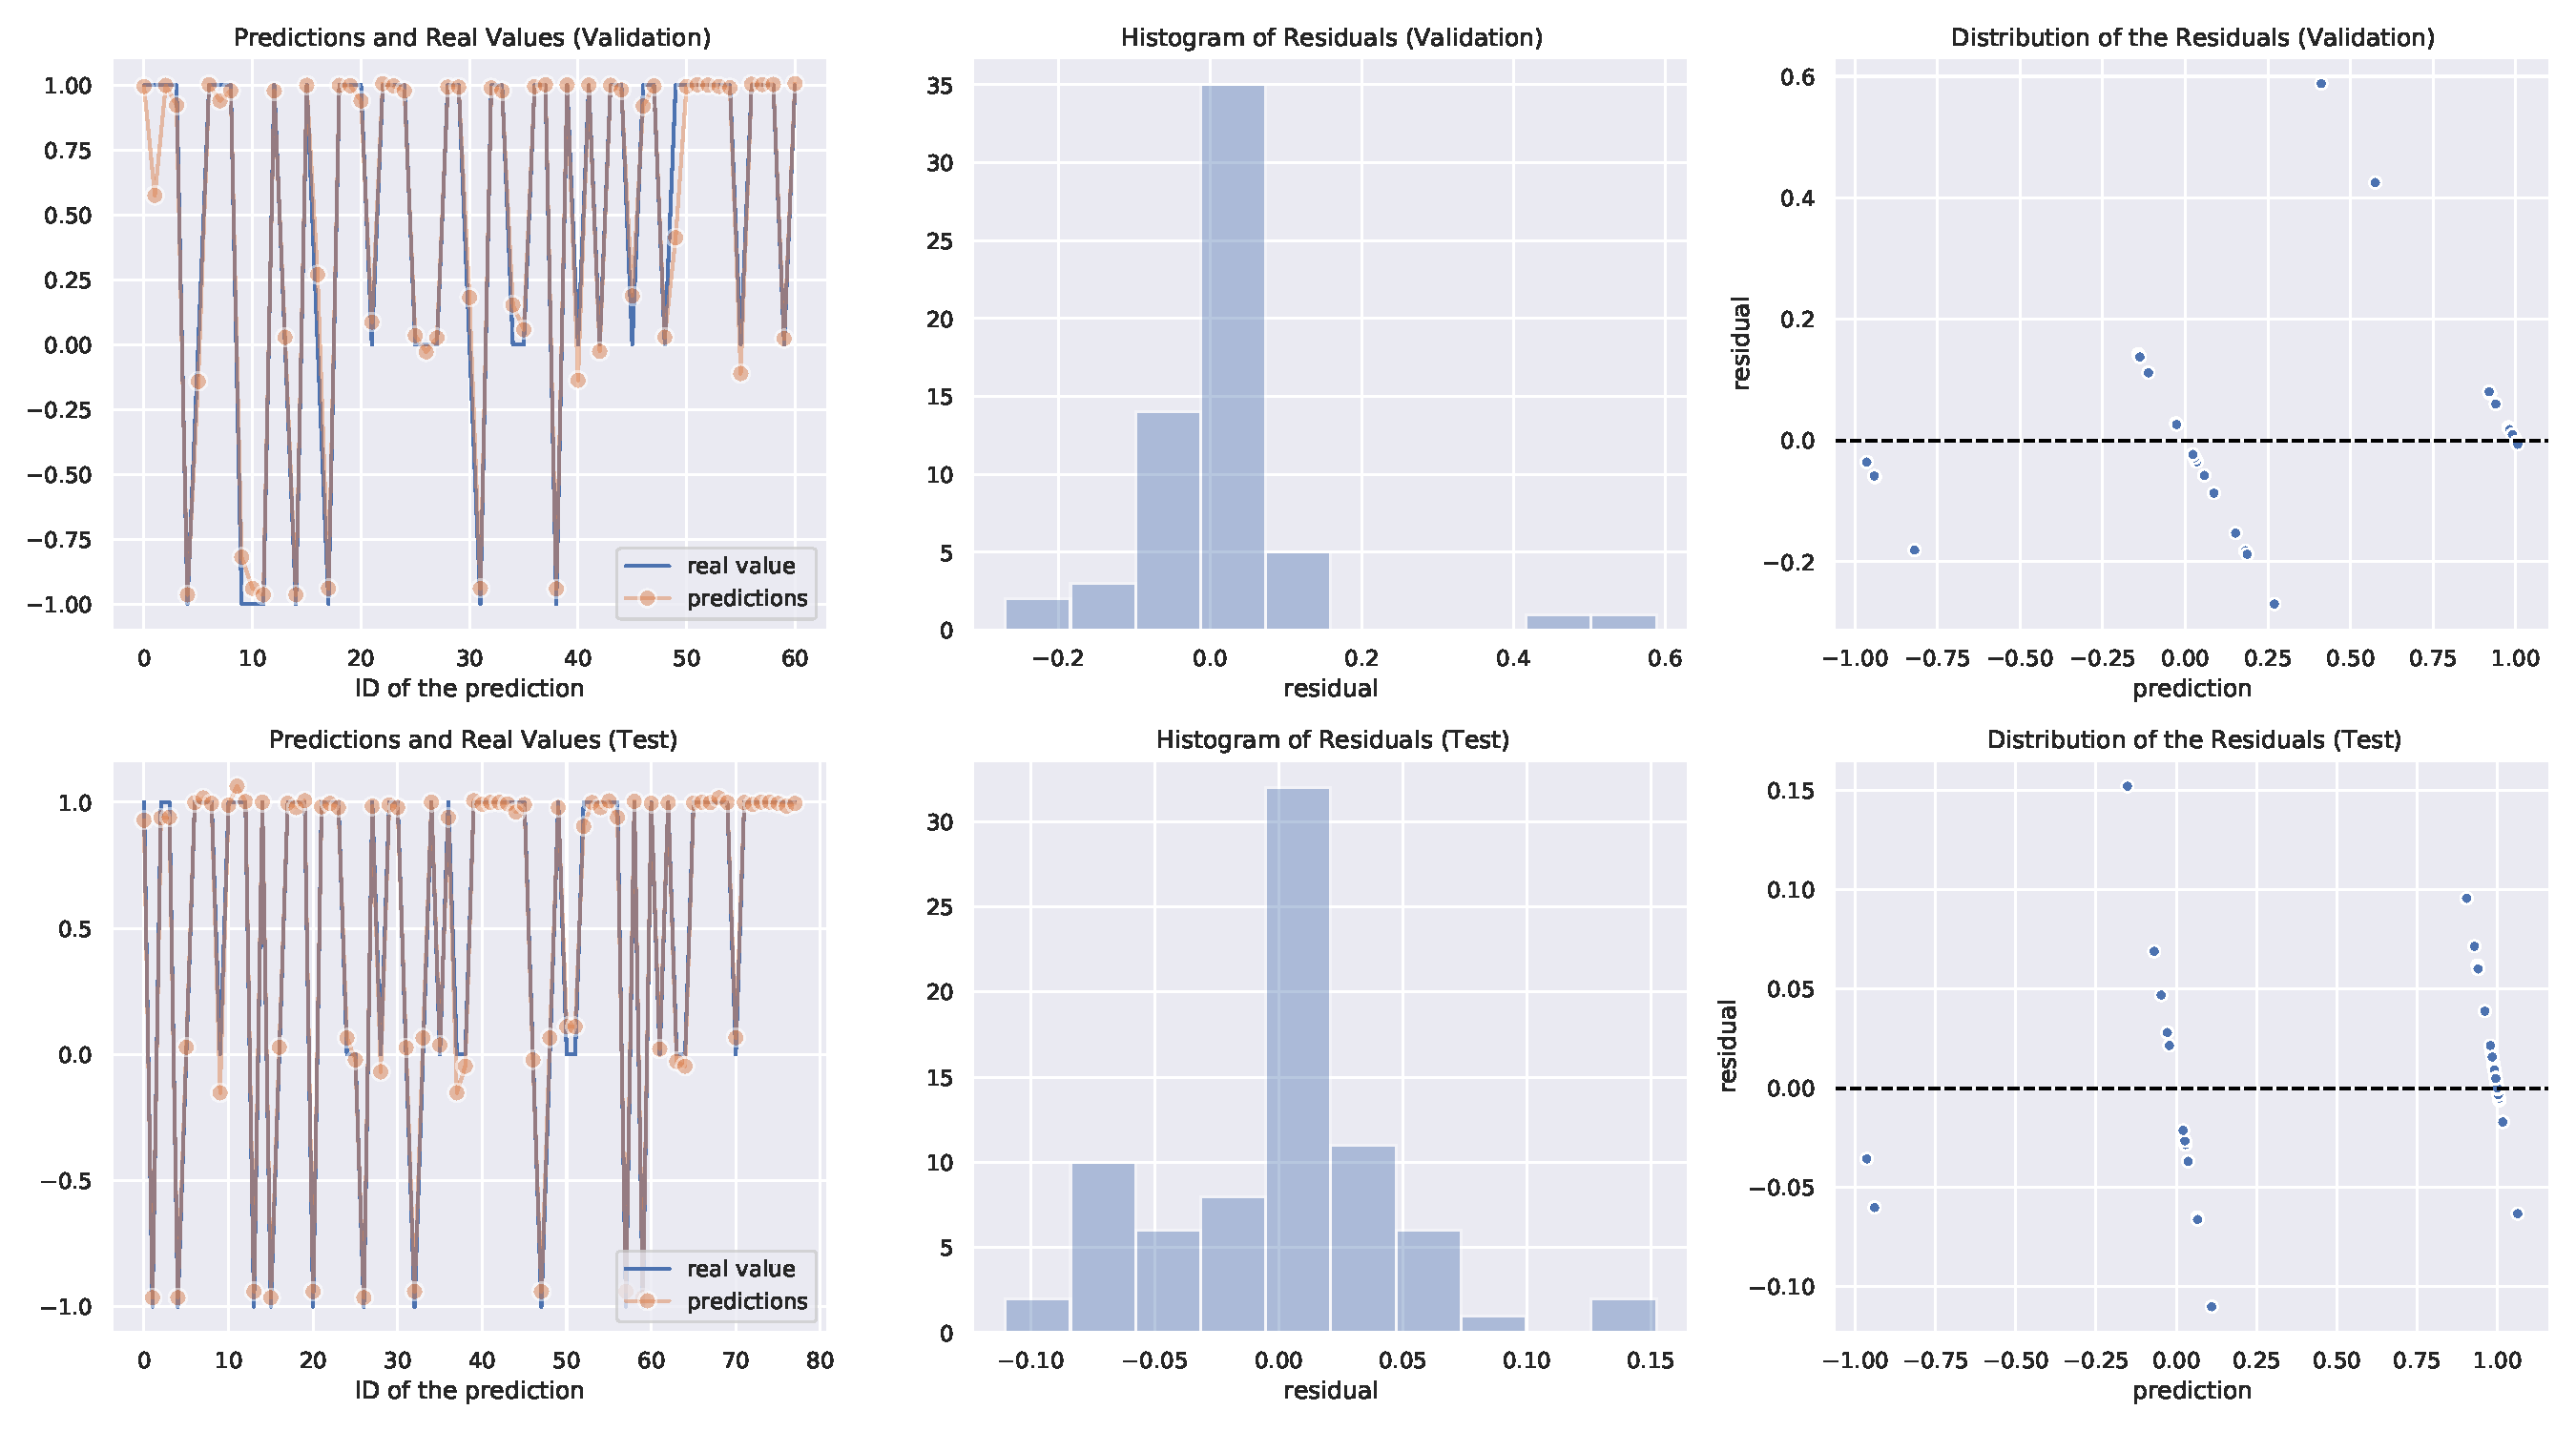
\includegraphics[width=0.475\textwidth]{img/grd_bst}
  \caption{GBDT validation and test sets residuals.
  When showing the predicted values compared to real values the markers show
  the position of the predictions and the line connecting then should help in
  following the sequence.
  True values are located at the angled points of the blue lines.}
  \label{fig:ml:gbdt}
\end{figure}

As we can see the GBDT are able to deliver the best results both in
terms of MSE and R2 score followed by the implementation of the shallow
network (trained over 5000 epochs: training is fairly rapid but trees are by
far faster).
On the other hand $\ell_1$ regularisation (both alone and in combination with
$\ell_2$) fails to approximate well the prediction labels. In the same fashion the
l-SVR fails completely.

In \Cref{fig:ml:gbdt} we show the validation and test set distribution of the
predictions and residuals.
As we can see the algorithm correctly approximates the \texttt{exp} labels with
residual contained in a small interval.
There is however a general tendency to underestimate the \texttt{exp} $= -1$
label and to overestimate \texttt{exp} $= 1$: in linear model this would have
signalled an incomplete model since residuals seem to be correlated with
predictions, but in the case of decision trees it does not pose an issue.

\begin{figure}[htbp]
  \centering
  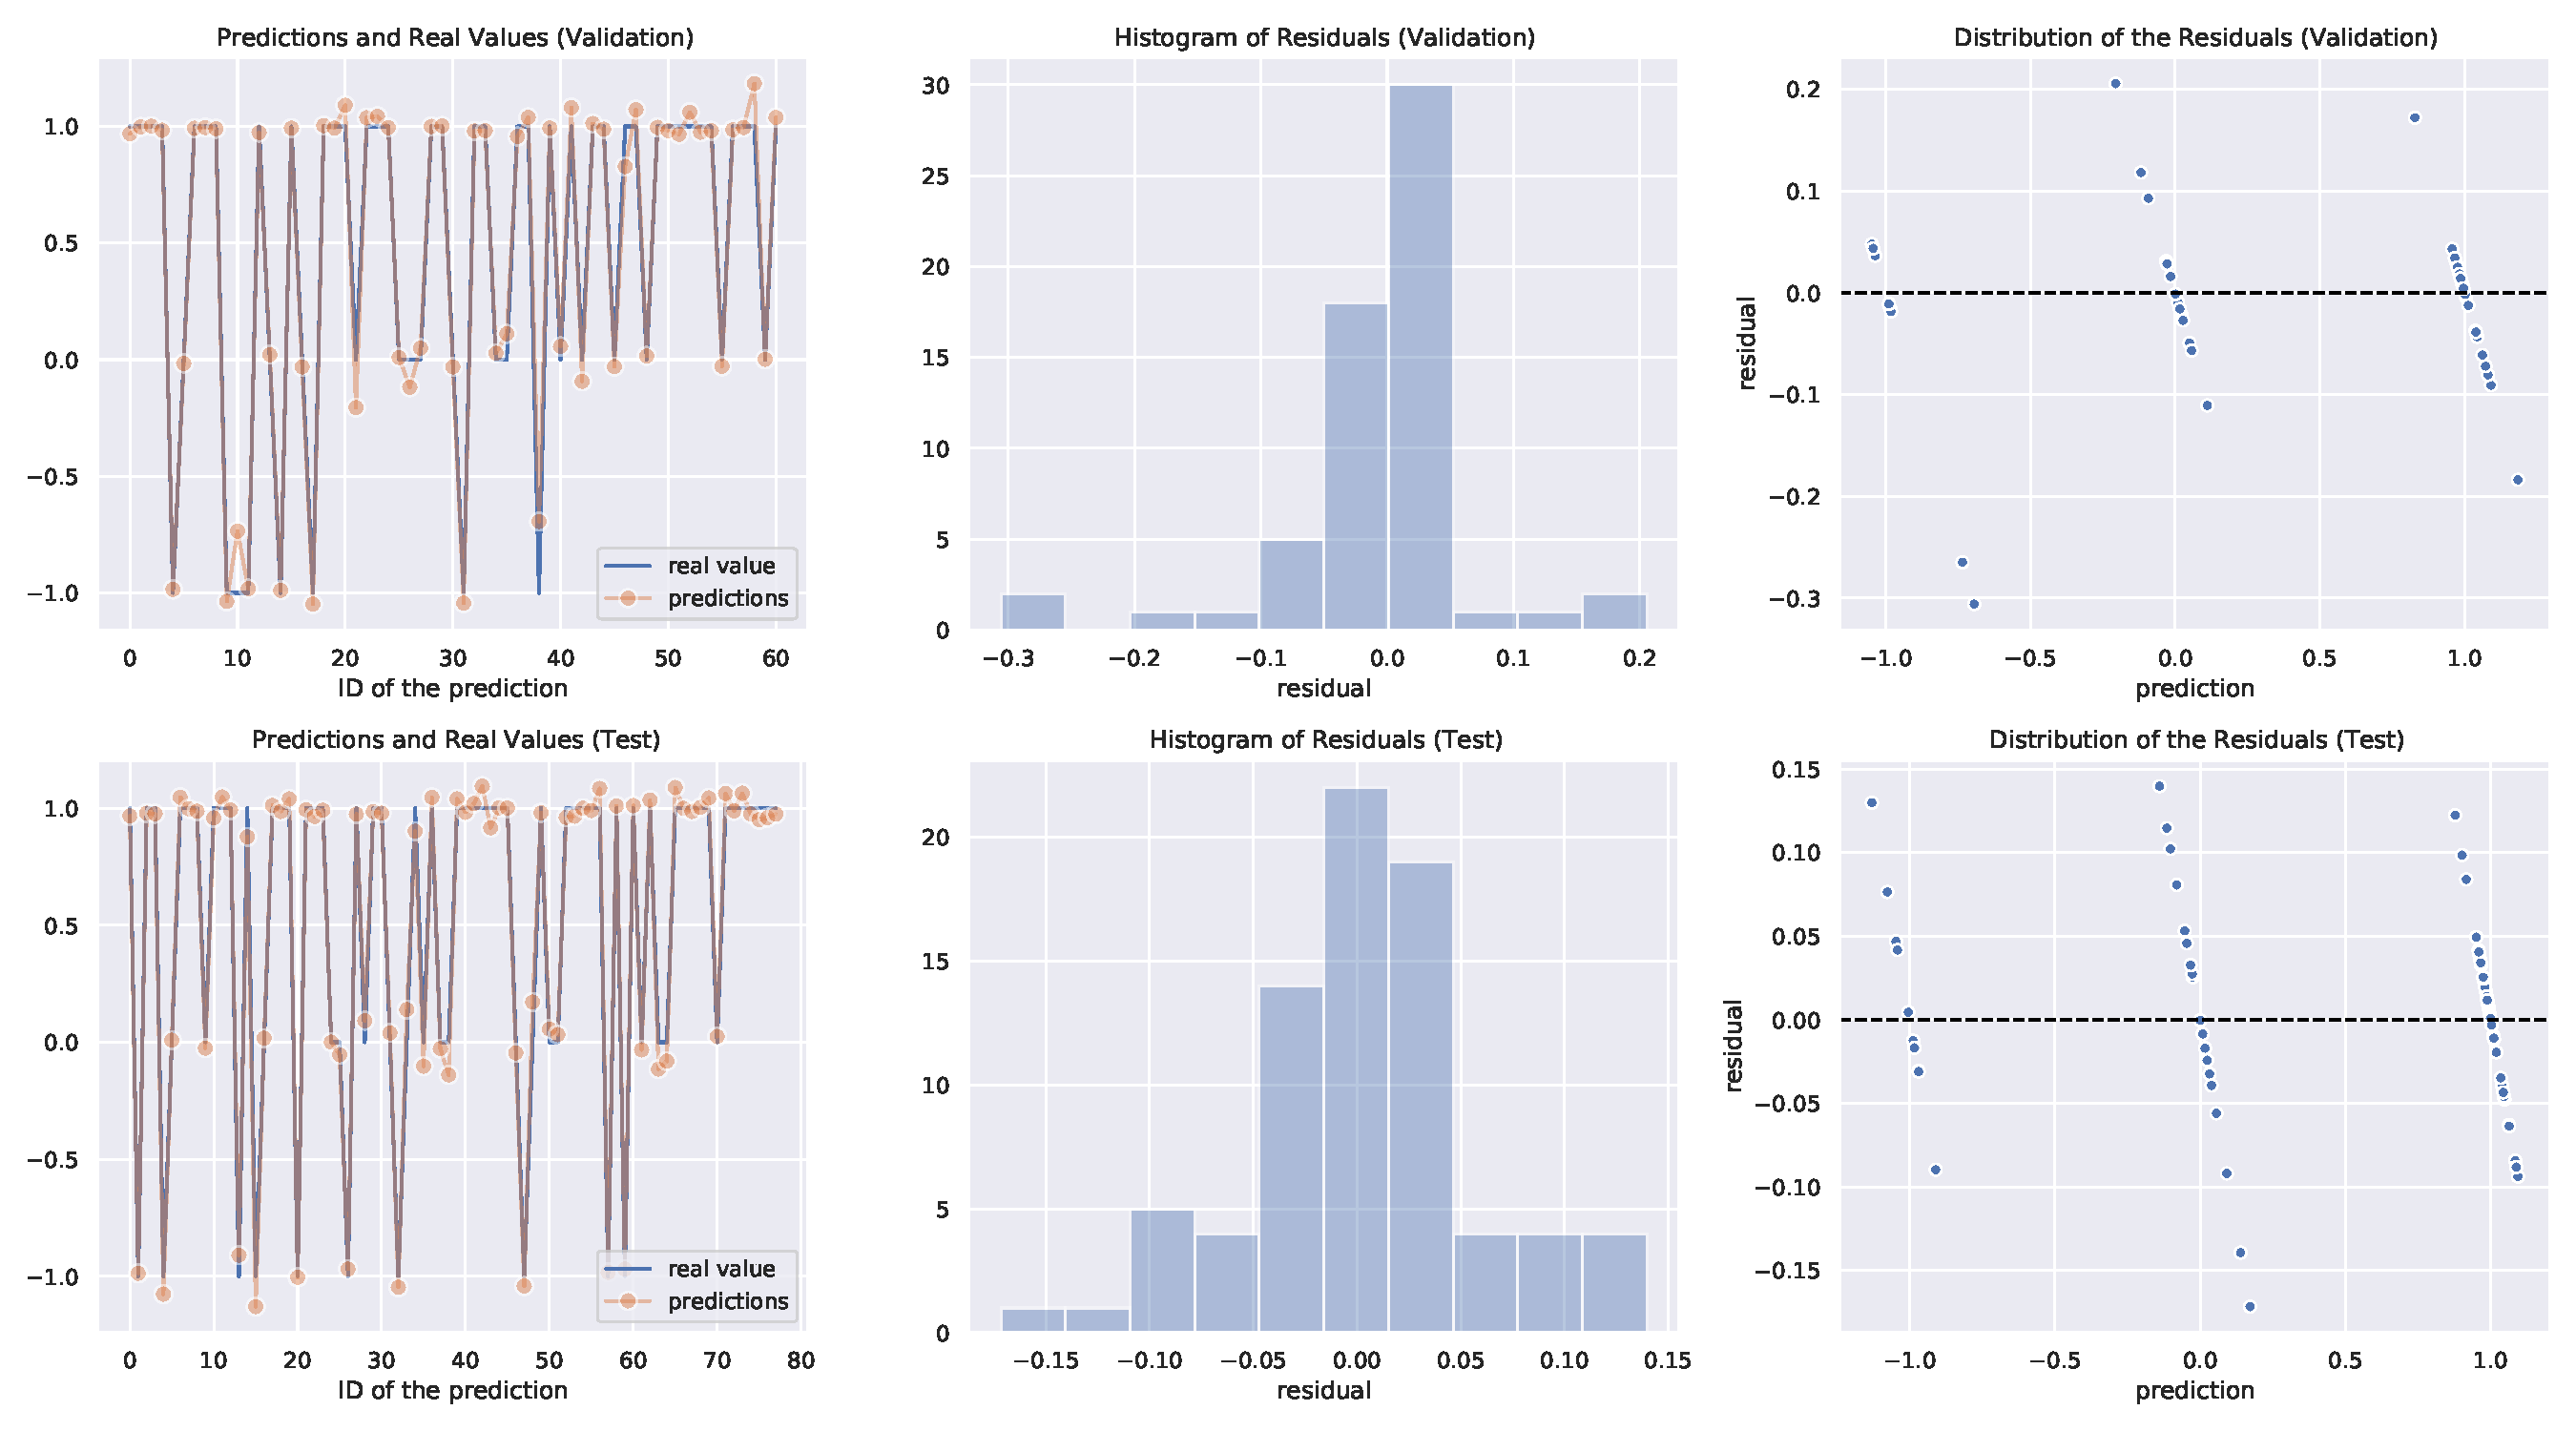
\includegraphics[width=0.475\textwidth]{img/ann_mod}
  \caption{ANN validation and test sets residuals.
  You can refer to the previous plot for an explanation of the graphical
  signs.}
  \label{fig:ml:ann}
\end{figure}

In \Cref{fig:ml:ann} we show the same plot generated from the ANN predictions.
As for the GBDT, the ANN is correctly trying to predict the \texttt{label} with
very small residuals.
Differently from the GBDT, residuals are more randomly distributed for each
prediction and no pattern is recognisable.

\begin{table}[htbp]
\centering
\begin{tabular}{@{}lcc@{}}
\toprule
                  & \textbf{RF} & \textbf{GBDT} \\
\midrule
no.\ leaves       & 48          & 25            \\
max depth         & 300         & 6             \\
no.\ estimators   & 25          & 3345          \\
subsample         & 0.85        & 0.99          \\
colsample by tree & 0.7         & 1.0           \\
min child weight  & 0.01        & 0.1           \\
$\ell_1$ reg.     & 0.16        & 2.1           \\
$\ell_2$ reg.     & 0.20        & 690           \\
learning rate     & ---         & 0.05          \\
\bottomrule
\end{tabular}%
\caption{Hyperparameters choices for RF and GBDT.}
\label{tab:ml:hyper}
\end{table}

In \Cref{tab:ml:hyper} we show a summary of the hyperparameters used for
training RF and GBDT: as expected the optimisation process chose a small number
of fully grown trees in the first case, while it led to a large number of
boosting rounds of shallow trees in the latter.

\subsection{Feature Explanation}\label{sec:ml:shap}

As a last step in the analysis, we use the trained trees (for simplicity) and
study their properties to possibly show how each training feature plays inside
the algorithm and how the final prediction is determined.
In this part of the analysis we study the variable ranking (i.e.\ the
importance of the features) provided by the binary structure of the trees and
the Shapley values~\cite{Lundberg:2017:Shap,Lundberg:2020:TreeExp} of each
feature.
The importance of the features is a key property of the decision trees and
visually summarises the impact that each feature has on the final prediction:
variables with higher importance can be found in the first branches of the
trees because they are responsible for the main choices of the algorithm, while
more negligible features provide the necessary refinement.
The Shapley values are somewhat related and derive from a game theoretic
approach to the decision trees: these values encode how a certain feature is
influencing the final result, whether by dragging its value with respect to
average of the predictions or by pushing it beyond it.
In other words, feature importances show how much (as a percentage of the final
prediction) a variable is relevant for the algorithm and the Shapley values
show if there are variables which tend to drive the results towards a
particular value (by computing the interaction between Shapley values we can
also try to recognise inter-dependencies inside the trees which may be worth
analysing further since the EDA could not have possibly picked them up, since
they are a product of the training process).

\begin{figure}[htbp]
  \centering
  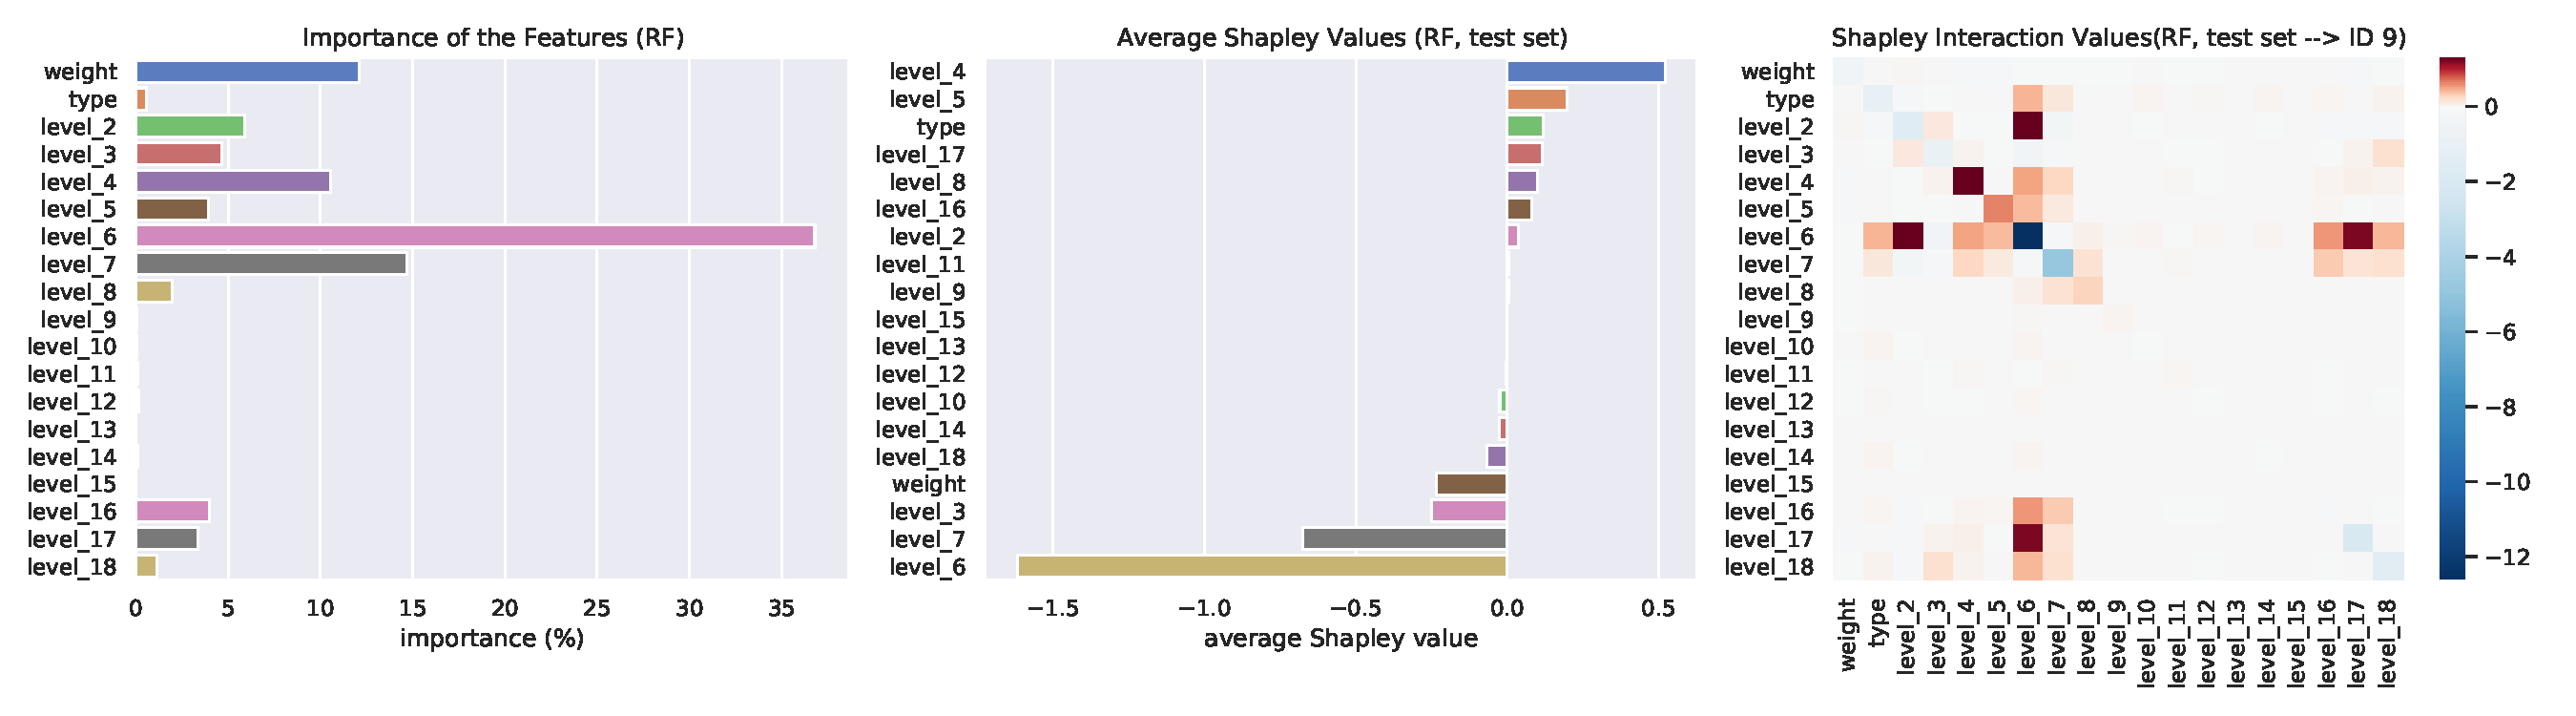
\includegraphics[width=0.475\textwidth]{img/rnd_for_shapley}
  \caption{Variable ranking and Shapley values (computed on the test set) of
  RF.}
  \label{fig:ml:rnd_for_shap}
\end{figure}

In \Cref{fig:ml:rnd_for_shap} we show the variable ranking and the Shapley
values for the RF algorithm.
The first plot sow that RF rely on a particular truncation level (level-6 to be
specific) to produce the predictions, while other features contribute in a less
relevant manner.
The average Shapley values (second plot) show that most features give a
comparable contribution to the prediction, exception made for the mass
truncation at level-6 and level-7 which seem to drive the final result in a
more direct way (according to \Cref{fig:eda:distr_full} they are among the
highly unbalanced values, which may be a reason of such behaviour).
Finally the \textit{interacting Shapley values} (taken for a random sample in
the test set) in the third plot show that the whole set of variables is mostly
non interacting except very sporadic contributions between distant levels.

\begin{figure}[htbp]
  \centering
  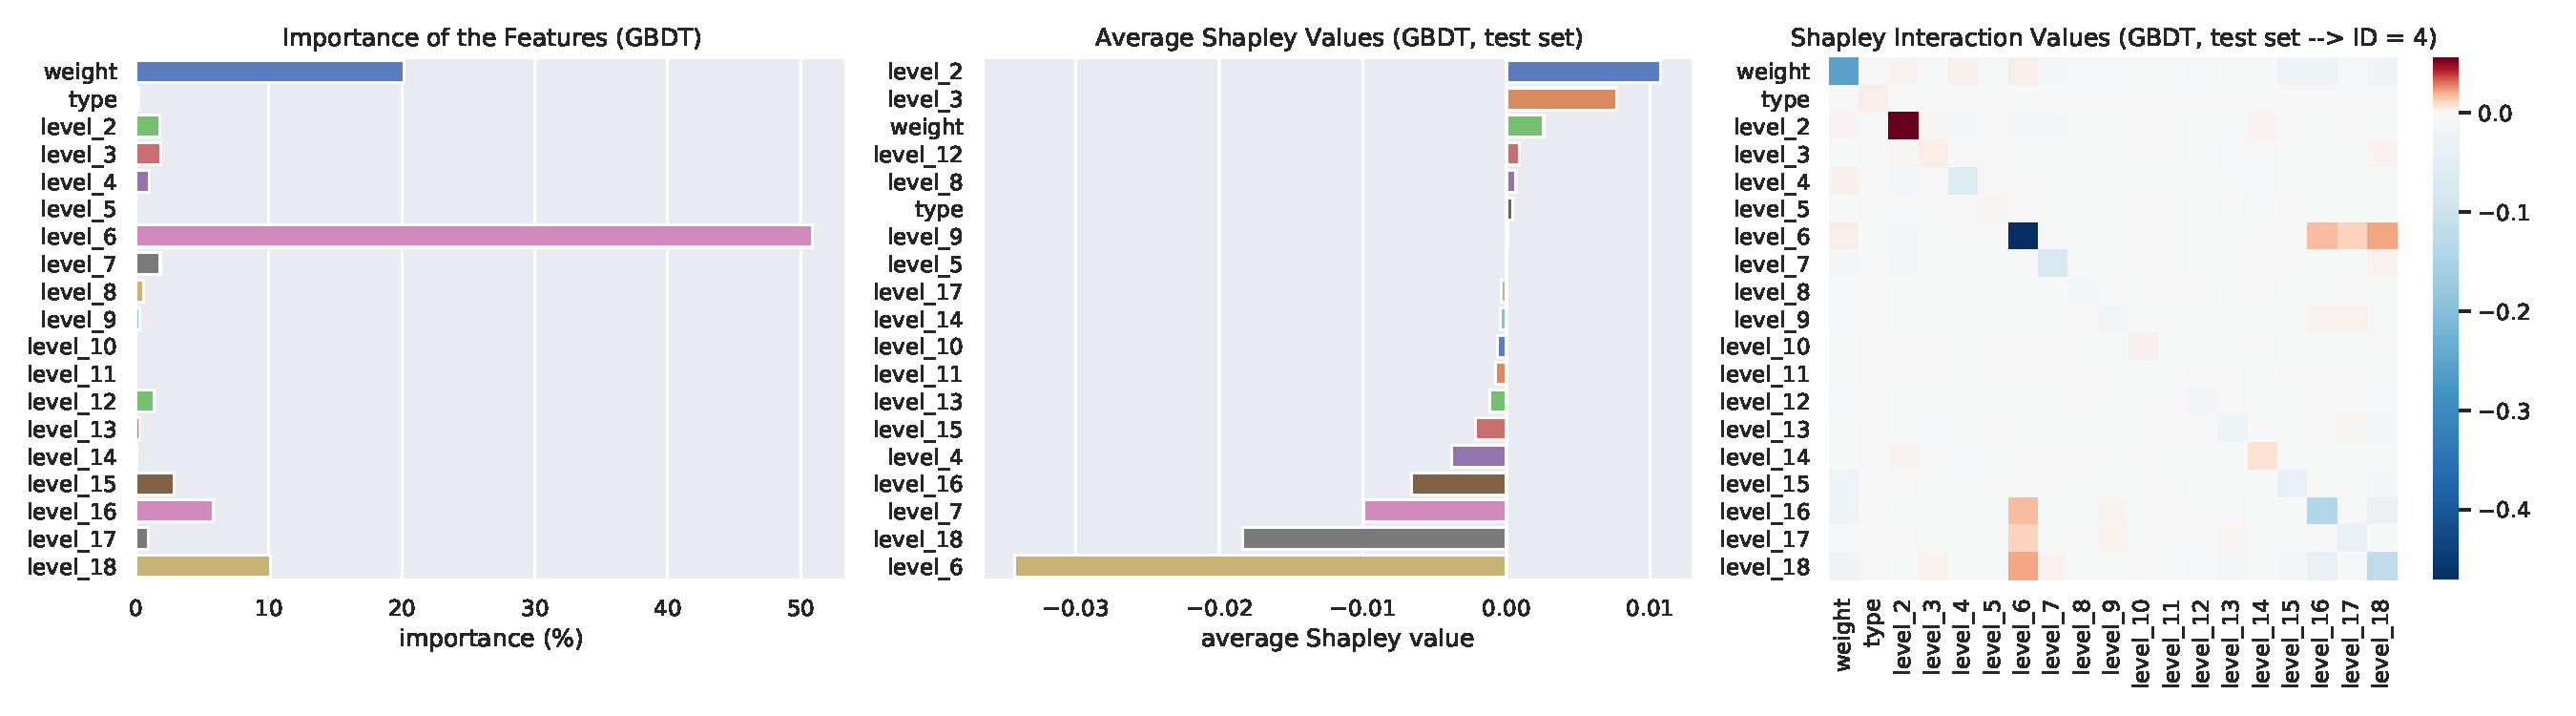
\includegraphics[width=0.475\textwidth]{img/grd_bst_shapley}
  \caption{Variable ranking and Shapley values (computed on the test set) of
  GBDT.}
  \label{fig:ml:grd_bst_shap}
\end{figure}

In \Cref{fig:ml:grd_bst_shap} we finally show the same plot for the GBDT.
Differently from the RF, GBDT seem to rely almost entirely on the 6th
truncation level and \texttt{weight} discrimination of the samples.

In both case the algorithms seem to ignore almost completely the categorical
variable \texttt{type} (possibly it could have been removed but the
corresponding Shapley value shows that its relevance is so marginal that the
result would not have changed).

We notice that the scale of the Shapley values is very different between RF and
GBDT: this is due to the fact that in this case the boosting procedure may be
more robust against the large variability of the dataset, showing that in the
GBDT case the trees are more balanced.
Ultimately this is also a consequence of the different order of magnitude of
the MSE associated to RF and GBDT, the latter being an entire order more
precise than the former.
